\subsection*{Иродов 2.28}

\setcounter{equation}{0}

\begin{abstract}
Грани полого куба заряжены равномерно с поверхностной плотностью $\sigma$. Найти силу, которая действует на каждую
грань со стороны:\\
а) точечного заряда $q$, если его поместить в центр куба;\\
б) остальных граней, если ребро куба равно $l$.
\end{abstract}

\noindent \hrulefill
\\
\begin{wrapfigure}[6]{r}{0.30\textwidth}
	\raisebox{0pt}[\dimexpr\height-4\baselineskip\relax]{
	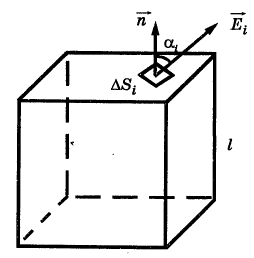
\includegraphics[width=0.30\textwidth]{pics/2_28.png}}
\end{wrapfigure}

а) Выберем плоскость Гаусса как замкнутый куб со стороной $r$, окружающий точечный заряд $q$.

По теореме Гаусса:

$$6\times E \times r^2=\frac{q}{\epsilon_{0}}\\ \xrightarrow{} E_(r) = \frac{q}{6\epsilon_0  r^2}$$

Вследствие симметрии компоненты $\overrightarrow{E}$ в направлении грани компенсируются. \\Сила на каждую грань:

$$F_1 = \sigma \times S \times E_(r=l) = \sigma \times l^2 \times \frac{q}{6\epsilon_0  l^2} = \frac{\sigma q}{6 \epsilon_0}$$

б) Согласно теореме Гаусса, поток в одном направлении создаваемый граней куба:

$$2 \times \Phi_1 = \frac{Q_1}{\epsilon_0} = \frac{\sigma l^2}{\epsilon_0} \xrightarrow{} \Phi_1 = \frac{\sigma l^2}{2 \epsilon_0}$$

Выберем плоскость Гаусса как замкнутый куб со стороной $r>l$, окружающий наш куб.

Поток через одну грань плоскость Гаусса:

$$6 \times \Phi = \frac{6 \times \sigma \times l^2}{\epsilon_0} \rightarrow \Phi = \frac{\sigma l^2}{\epsilon_0}$$

$\Phi' - $ поток, создаваемый остальными гранями.

$$\Phi = \Phi' + \Phi_1 \\ \rightarrow \Phi' = \Phi - \Phi_1 = \frac{\sigma l^2}{2 \epsilon_0}$$

Сила на одну грань остальными гранями:

$$F_2 = Q \times E' = \sigma \times S \times E' = \sigma \times \Phi' = \frac{\sigma^2 l^2}{2 \epsilon_0}$$

\textbf{Ответ:}
$$F_1 = \frac{\sigma q}{6 \epsilon_0}$$ 
$$ F_2 = \frac{\sigma^2 l^2}{2 \epsilon_0}$$





